\chapter{Futuras Líneas de Trabajo}

Durante el desarrollo de este Trabajo de Fin de Grado se han podido completar la mayoría de los objetivos y requisitos del sistema que se propusieron, pero hay otros que han quedado sin completar. También, aunque no estuviesen pensadas en un principio, han ido surgiendo ideas que aportaban valor al proyecto.

\section{Posibles mejoras}

\subsection{Mejoras en la API REST}

La principal característica a incluir en la API es la seguridad. En este momento, cualquiera puede realizar un POST sobre la base de datos, algo que desde el punto de vista de la seguridad informática, no es nada seguro. A continuación se expondrá una posible solución a este problema, como es la utilización de tokens como medida de seguridad.

\subsubsection{JSON Web Tokens}

Se trata de un estándar que describe un mecanismo para difundir información de forma segura entre dos partes, incluyendo en objectos de tipo JSON parámetros como la identidad de un usuario o los privilegios del mismo.

El web token es una cadena de texto codificado en Base64 \cite{josefsson2006base16} con tres partes claramente diferenciadas y separadas por un punto. Como la que se muestra en la siguiente figura \ref{fig:JWT}

\begin{figure}[H]
    \centering
    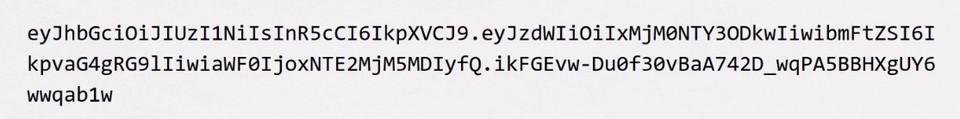
\includegraphics[width=\textwidth]{include/figuras/JWT.jpg}
    \caption{JSON Web Token}
    \label{fig:JWT}
\end{figure}

Como hemos explicado anteriormente, cada token está compuesto por tres partes distintas

\begin{itemize}
    \item \textbf{Header}: es el encabezado del token, en él se especifica el tipo de token y el algoritmo de codificación que se utiliza.
    \item \textbf{Payload}: es la zona en la que aparecen los distintos datos del usuario y los privilegios del mismo. Además se puede añadir tanta información como se crea necesario.
    \item \textbf{Signature}: firma que indica si el token proporcionado es válido o no. Se construye de tal manera, que es posible comprobar de manera sencilla si el token ha sido modificado por el camino.
\end{itemize}

Tanto el payload como el header se codifican en Base64, a estos dos se les añade un secreto establecido por la aplicación. De forma que si detectamos la modificación del token sea sencillo rechazar esa petición.

\subsection{Filtros}

La API REST tiene implementados distintos filtros para obtener información, pero desde el equipo del proyecto se ha especificado que sería conveniente la posible concatenación de distintos filtros. 
Para que quede más claro utilizaremos un ejemplo:

Ahora mismo, es posible obtener un eco determinado en base a su \textit{identificador}, y también obtener uno aleatorio mediante el quer yparam \textit{?policy=random}. 
Al realizar distintas pruebas, el equipo consideró necesario la implementación de filtros por tipo de eco, por duración o por la cantidad de clasificaciones que ha sufrido dicho elemento.

\section{Mejoras del chatbot}

Como principal mejora del chatbot, sería la de darle la capacidad al asistente de poder comunicarse y recibir la información a través de la utilización de la voz. De esta forma, proporcionamos acceso a la aplicación a personas que tienen algún tipo de disfunción visual o no dominan la lectoescritura.

También sería conveniente proporcionarle la capacidad de comunicación en otros idiomas, sobretodo el inglés, para que la base de usuarios crezca exponencialmente.

\section{Futuros proyectos}

Durante la realización de este trabajo de fin de grado surgieron algunas ideas sobre futuros proyectos establecidos dentro del marco de Sonidos del Cielo como la idea de la creación de un Dashboard para análisis de los datos de las clasificaciones realizadas.